\documentclass[border=10pt]{standalone}
\usepackage{pgfplots}
\pgfplotsset{compat=1.18}
\begin{document}
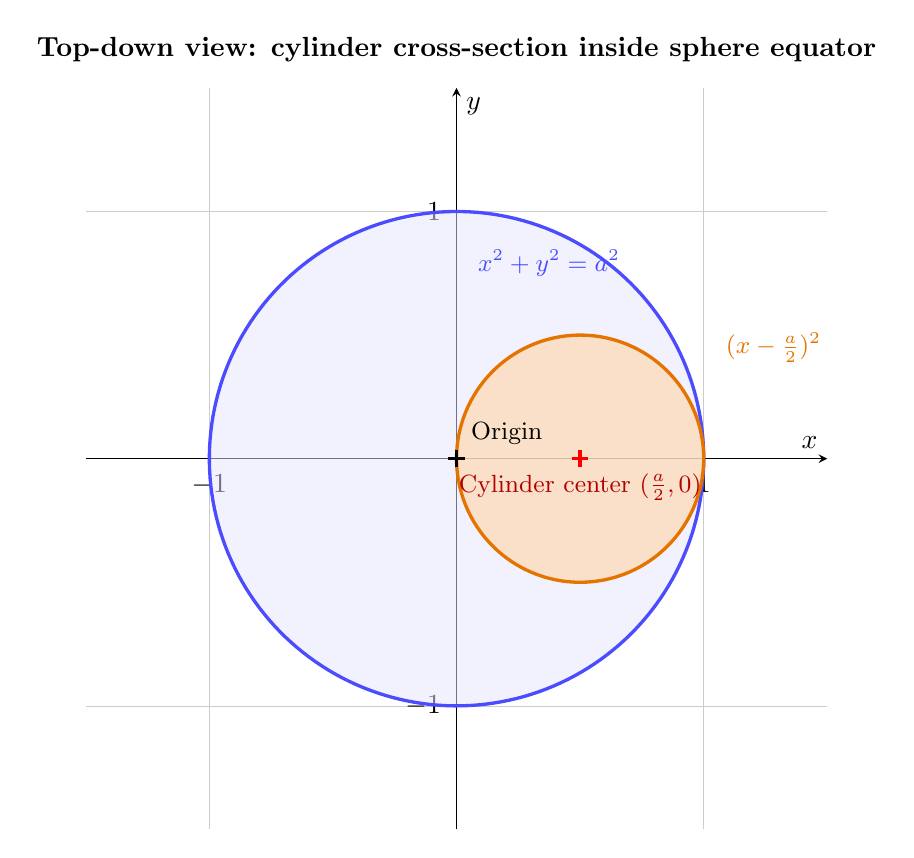
\begin{tikzpicture}
\begin{axis}[
    width=11cm, height=11cm,
    axis equal image,
    xlabel={$x$}, ylabel={$y$},
    xmin=-1.5, xmax=1.5,
    ymin=-1.5, ymax=1.5,
    xtick={-1,0,1}, ytick={-1,0,1},
    grid=both, major grid style={line width=.2pt,draw=gray!40},
    axis lines=middle,
    title={Top-down view: cylinder cross-section inside sphere equator},
    title style={align=center, font=\bfseries},
]

% Outer disk (sphere equator) - light blue fill + outline
\addplot[
    domain=0:360, samples=200, draw=blue!70, very thick,
    fill=blue!10, fill opacity=0.5,
] ({cos(x)},{sin(x)}) -- cycle;

% Cylinder cross-section disk - light orange fill + outline
\addplot[
    domain=0:360, samples=200, draw=orange!90!black, very thick,
    fill=orange!30, fill opacity=0.7,
] ({0.5+0.5*cos(x)},{0.5*sin(x)}) -- cycle;

% Mark the two centers
\addplot[only marks, mark=+, mark size=3pt, very thick, black] coordinates {(0,0)};
\addplot[only marks, mark=+, mark size=3pt, very thick, red]  coordinates {(0.5,0)};

% Labels
\node[anchor=south west, font=\small] at (0.02,0.02) {Origin};
\node[anchor=north, font=\small, red!70!black] at (0.5,-0.02) {Cylinder center $(\frac{a}{2},0)$};

% Tick labels
\node[anchor=south east, font=\small, blue!70] at (0.7,0.7) {$x^2+y^2=a^2$};
\node[anchor=west,       font=\small, orange!90!black] at (1.05,0.45) {$(x-\frac{a}{2})^2+y^2=(\frac{a}{2})^2$};

\end{axis}
\end{tikzpicture}
\end{document}
